\documentclass{article}
\usepackage[utf8]{inputenc}
\usepackage{graphicx,caption}
\graphicspath{ {./images/} }
\usepackage{float}
\usepackage{caption}
\usepackage{subcaption}
\usepackage[unicode]{hyperref}
\usepackage{amsmath}

\title{Homework 2 - Laboratory}
\author{Dainese Fabio, 857661}
\date{March 15, 2020}

\begin{document}

\maketitle

\section{Giant Component}
    By filtering out the Giant component, applying Force Atlas 2 layout (scaling 2.0 and gravity 10.0) and coloring the nodes following the node-partition the result obtained in Gephy is the following:

    \begin{figure}[H]
        \centering
        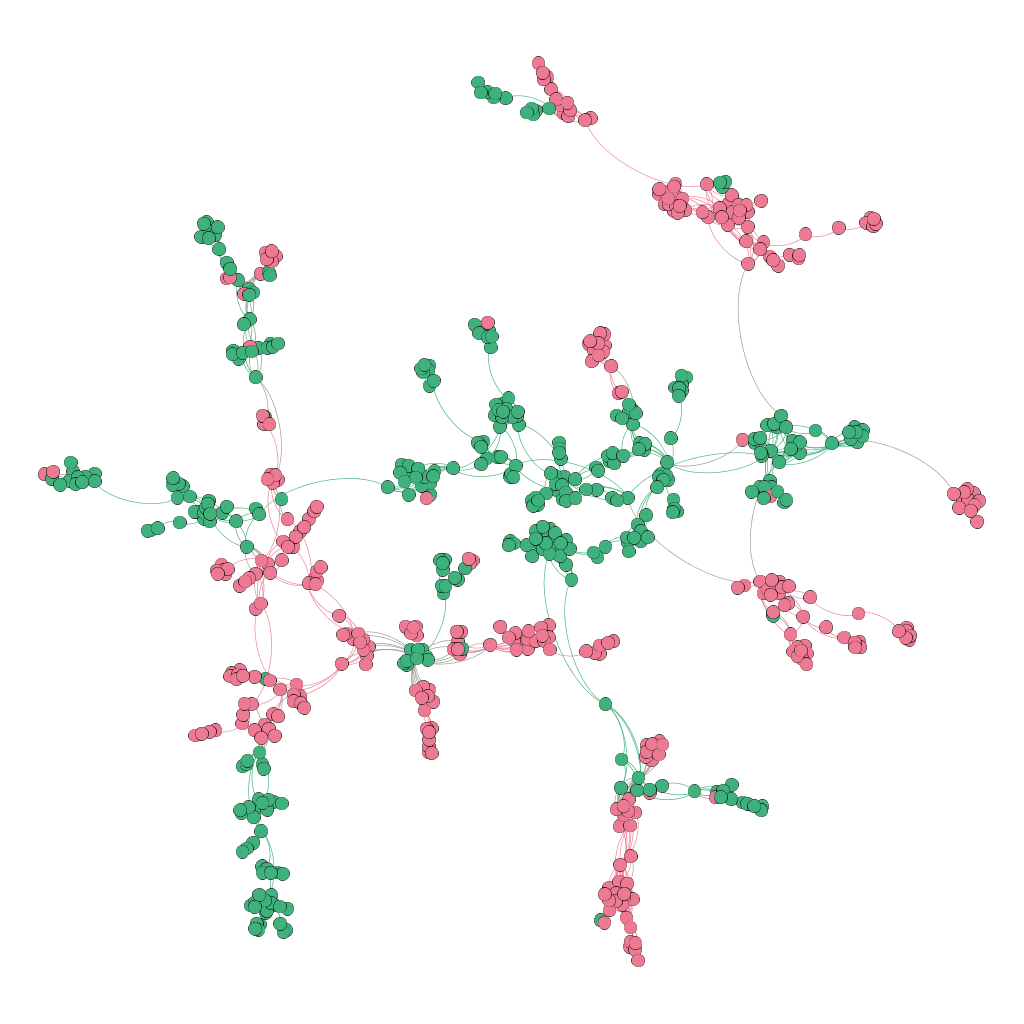
\includegraphics[width=0.6\textwidth]{1.0.png}
        \caption{Giant component}
        \label{fig:figure-1}
    \end{figure}
    
    \noindent Moreover, if we apply also the 'Dissuade Hubs', 'LinLog Mode' and 'Prevent Overlap' options we obtain a more readable graph like the one reported in the 'Figure \ref{fig:figure-1.1}'.
    
    \begin{figure}[H]
        \centering
        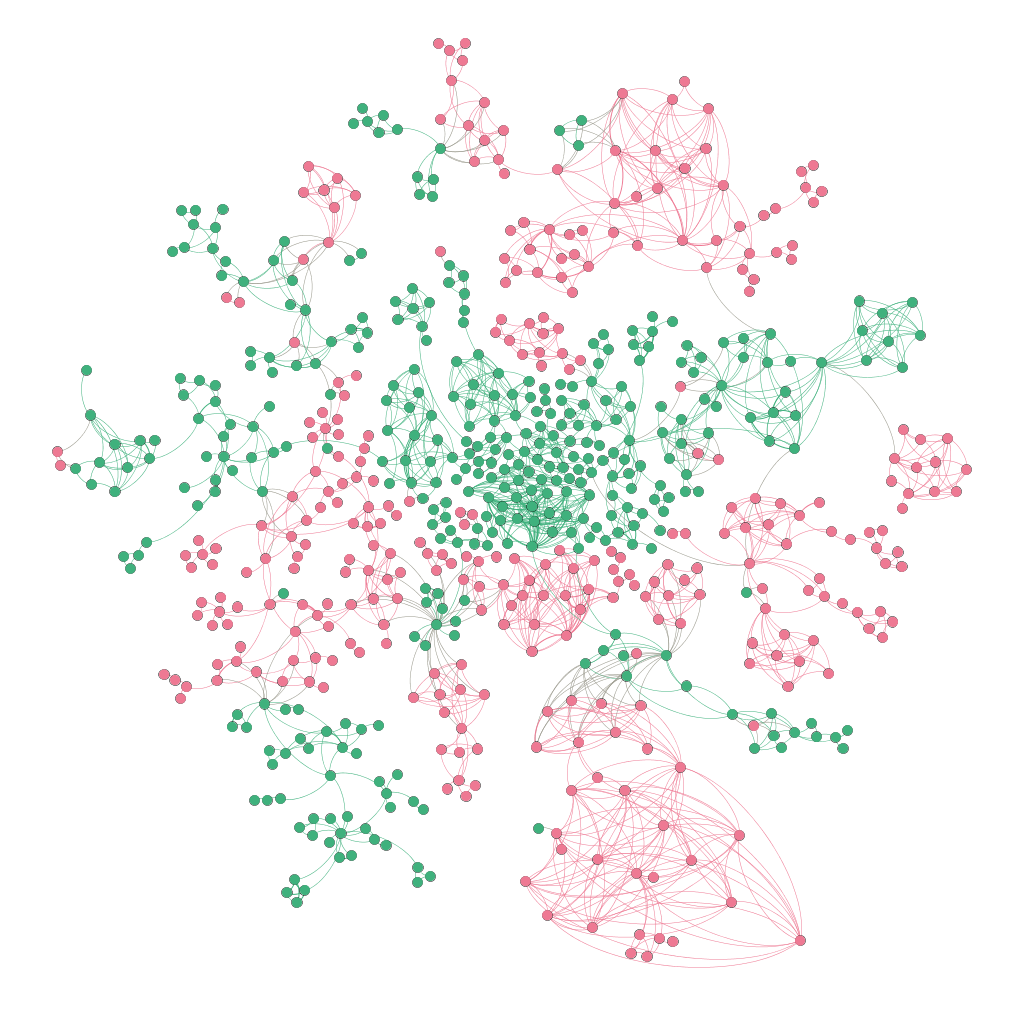
\includegraphics[width=0.6\textwidth]{1.1.png}
        \caption{Giant component}
        \label{fig:figure-1.1}
    \end{figure}

    \noindent In this situation by keeping the Giant-component filter running and creating a new workspace with the given subgraph, we have that: 

    \begin{enumerate}
        \item The number of nodes are 680, meanwhile the number of edges are 1887
        \item The average degree is 5.55
        \item The average path length is 12.005
        \item The maximum degree is 30 (ID: 87996)
        \item By putting in red color the depth-2 ego network of the node 87996 we obtain the following result:
        \begin{figure}[H]
            \centering
            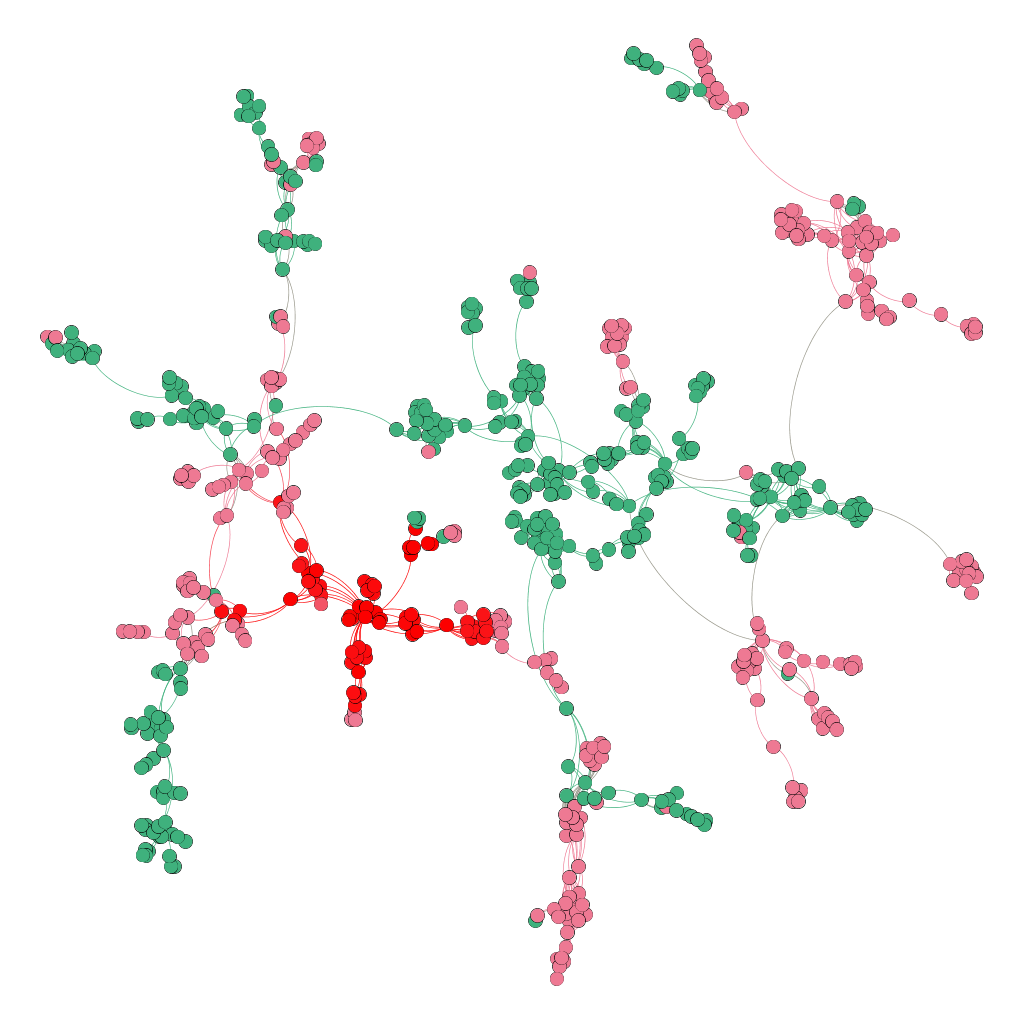
\includegraphics[width=0.6\textwidth]{2.0.png}
            \caption{Giant component with red depth-2 ego network of the node 87996}
            \label{fig:figure-2.0}
        \end{figure}
        \noindent Just for clarity, here's the isolated depth-2 ego network of the node 87996:
        \begin{figure}[H]
            \centering
            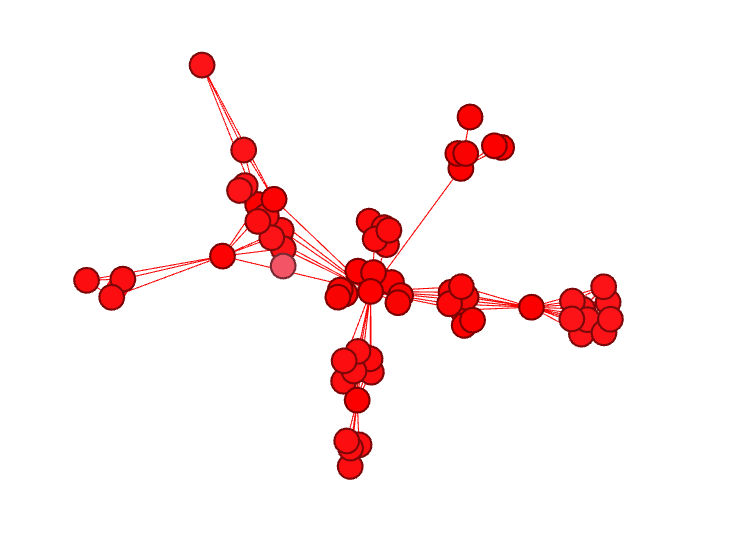
\includegraphics[width=0.5\textwidth]{2.1.png}
            \caption{Isolated depth-2 ego network of the node 87996}
            \label{fig:figure-2.1}
        \end{figure}
    \end{enumerate}

    \bigskip
    
    \noindent In this next paragraph you can look at some scatter plots that compares the degree of a node with the eigenvector centrality, closeness centrality and eccentricity.

    \begin{figure}[H]
        \centering
        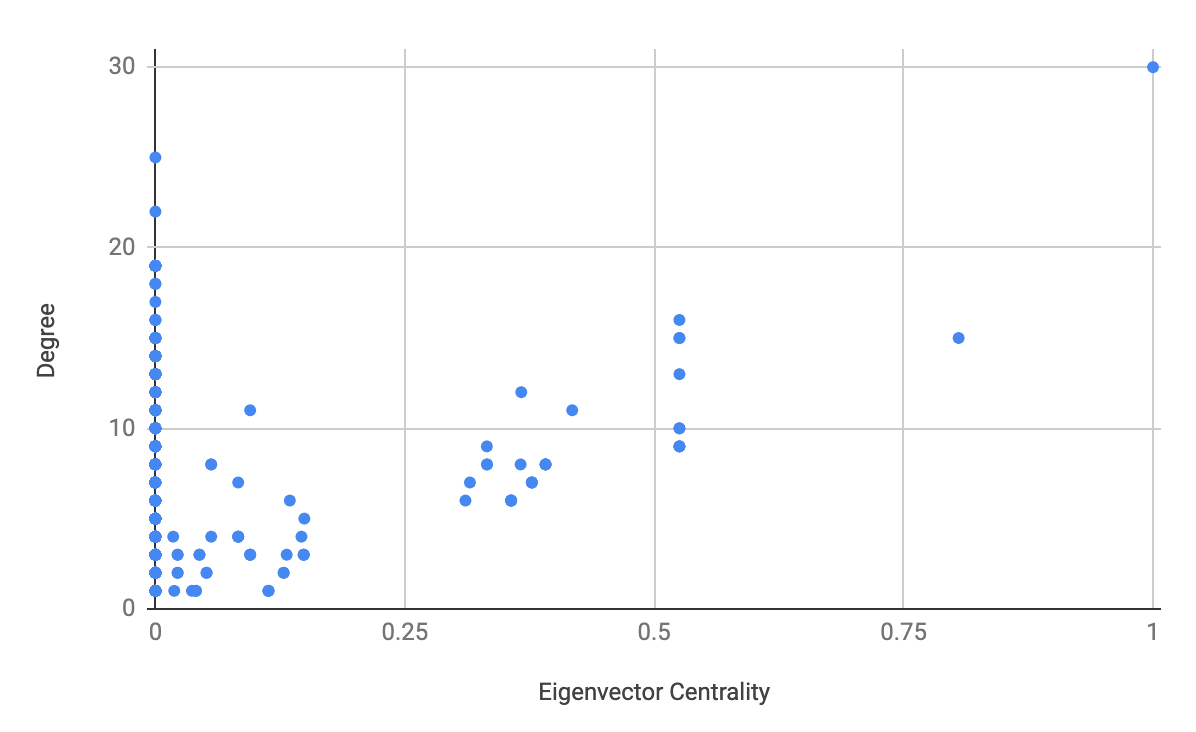
\includegraphics[width=0.7\textwidth]{3.1.png}
        \caption{Degree versus eigenvector centrality}
        \label{fig:figure-3.1}
    \end{figure}
    
    \begin{figure}[H]
        \centering
        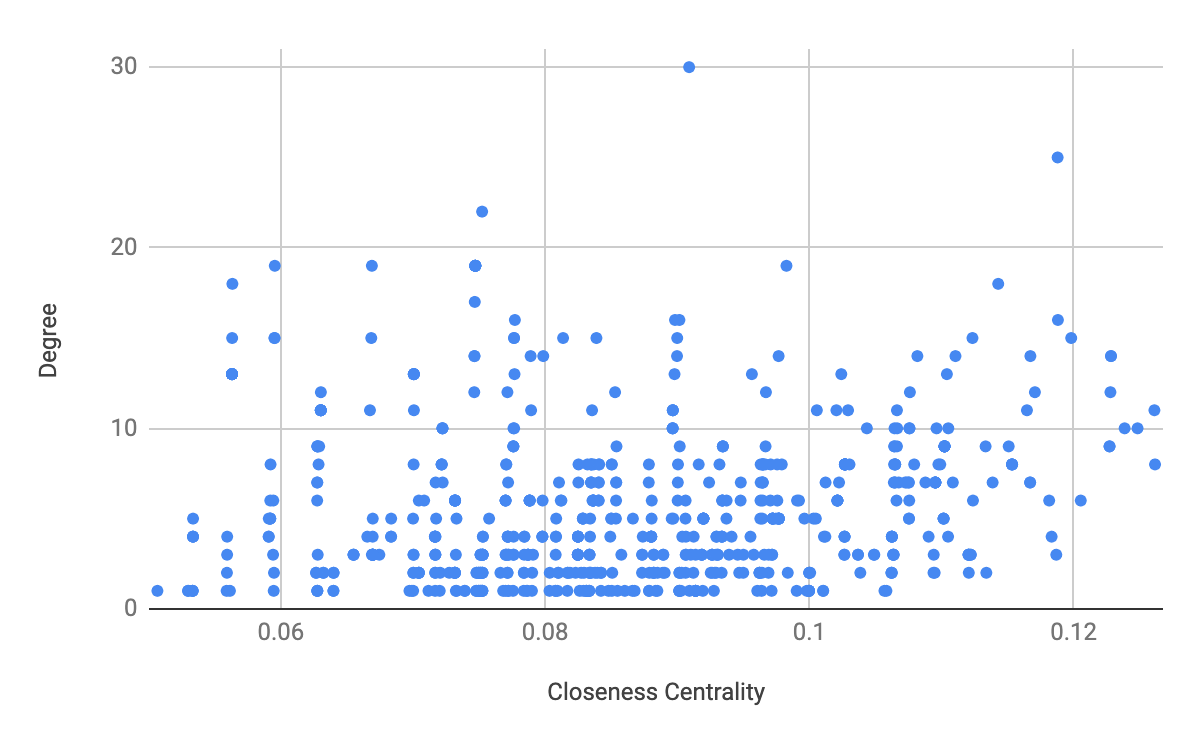
\includegraphics[width=0.7\textwidth]{3.2.png}
        \caption{Degree versus closeness centrality}
        \label{fig:figure-3.2}
    \end{figure}
    
    \begin{figure}[H]
        \centering
        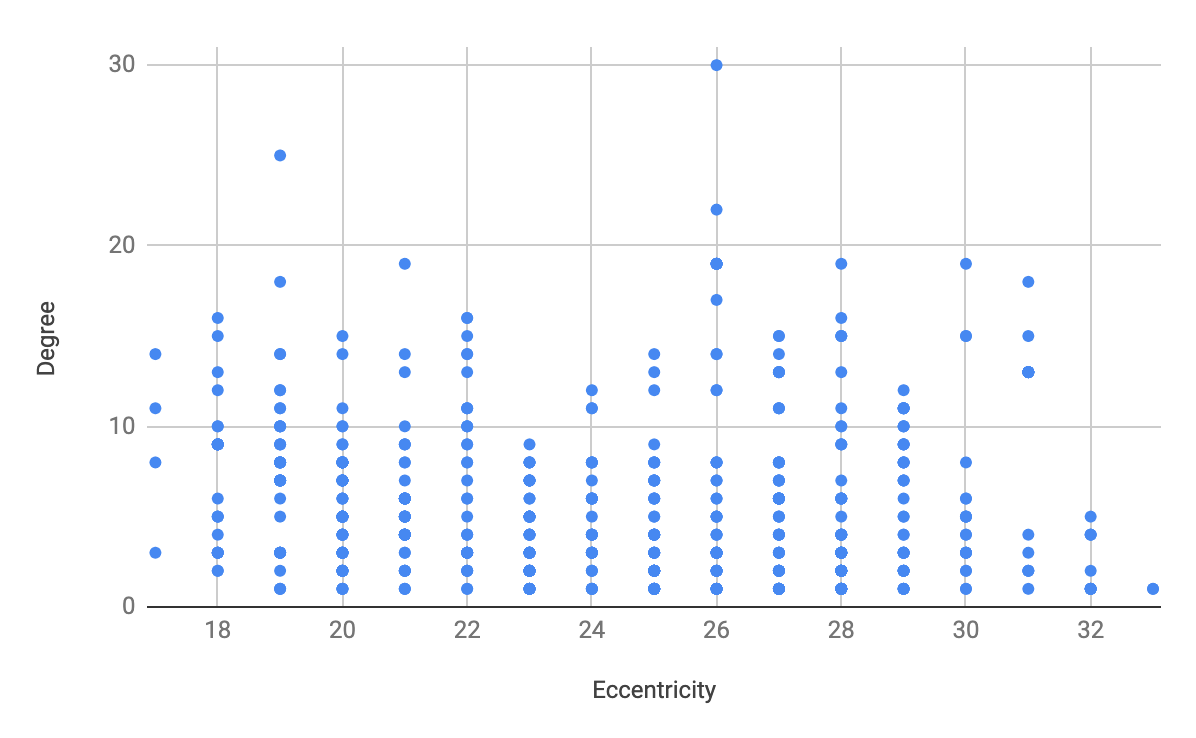
\includegraphics[width=0.7\textwidth]{3.3.png}
        \caption{Degree versus eccentricity}
        \label{fig:figure-3.3}
    \end{figure}

    \bigskip
    \noindent The next graphs are multiple representation of the Giant component with node size between 1 and 10 regarding different variables.
    
    \begin{figure}[H]
        \centering
        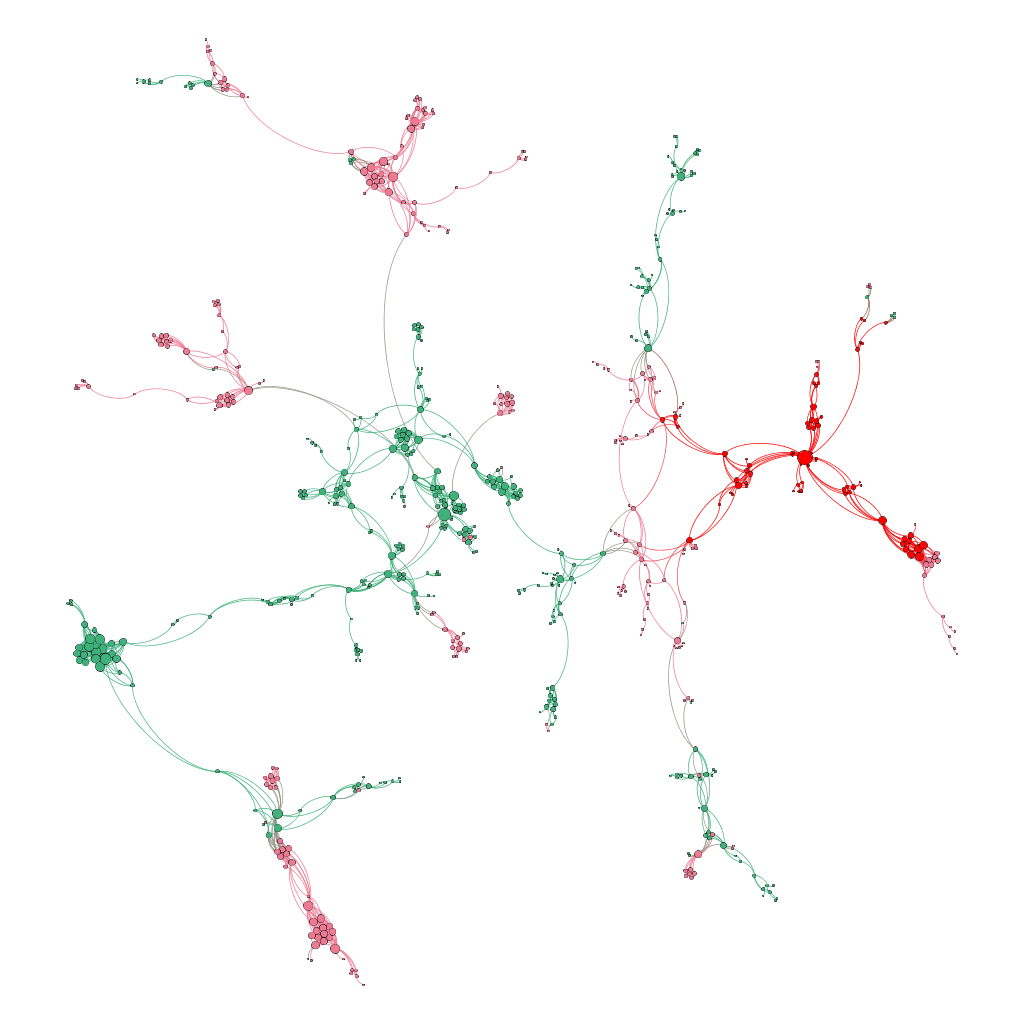
\includegraphics[width=0.55\textwidth]{4.1.png}
        \caption{Node size depending on the degree}
        \label{fig:figure-4.1}
    \end{figure}
    \begin{figure}[H]
        \centering
        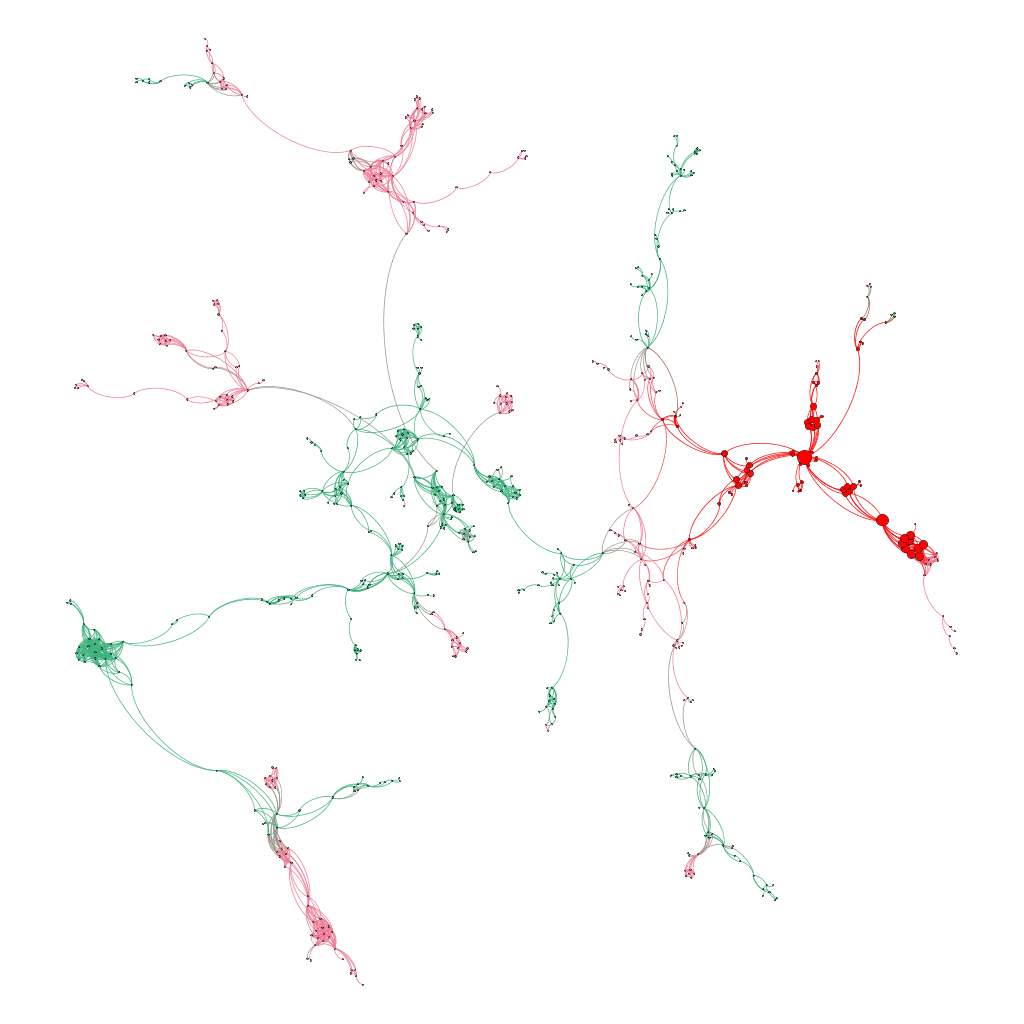
\includegraphics[width=0.52\textwidth]{4.2.png}
        \caption{Node size depending on the eigenvector centrality}
        \label{fig:figure-4.2}
    \end{figure}
    \begin{figure}[H]
        \centering
        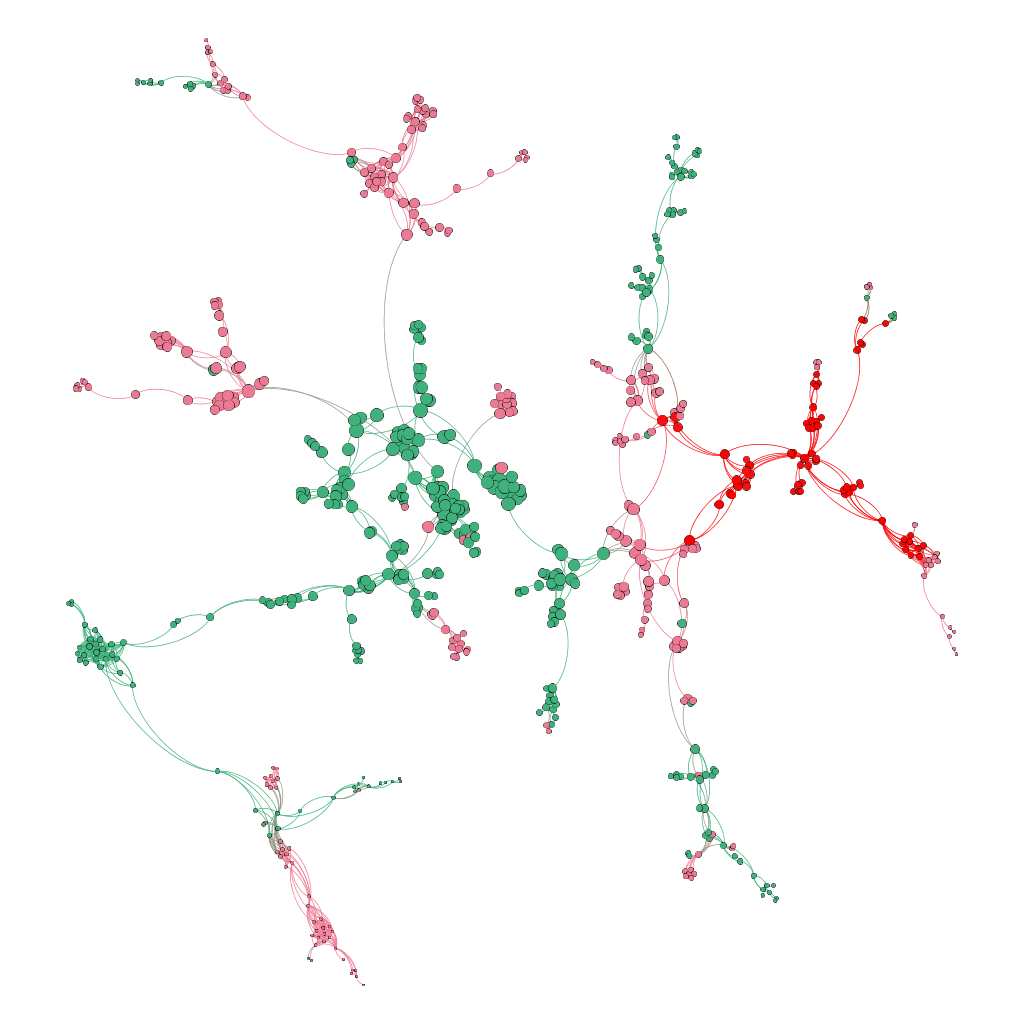
\includegraphics[width=0.52\textwidth]{4.3.png}
        \caption{Node size depending on the closeness centrality}
        \label{fig:figure-4.3}
    \end{figure}
    \begin{figure}[H]
        \centering
        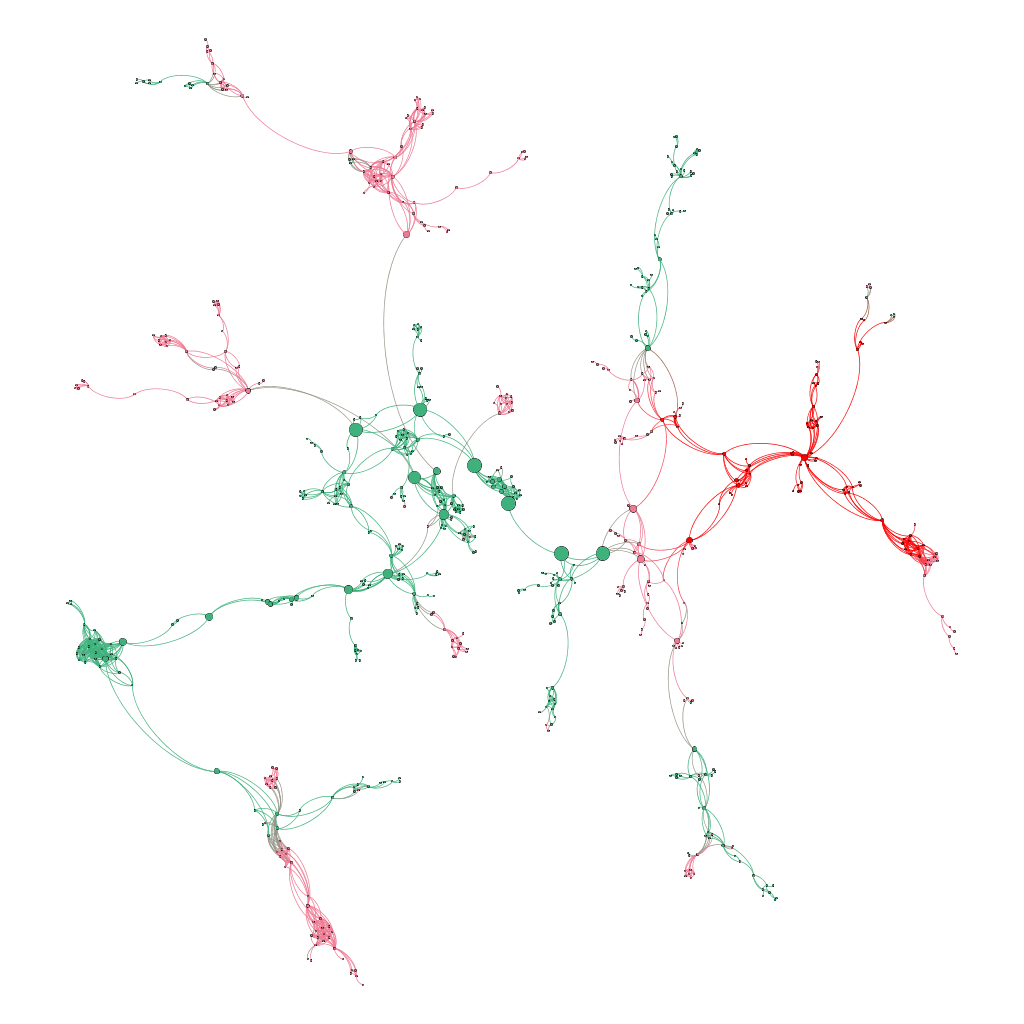
\includegraphics[width=0.52\textwidth]{4.4.png}
        \caption{Node size depending on the betweenness centrality}
        \label{fig:figure-4.4}
    \end{figure}
    \begin{figure}[H]
        \centering
        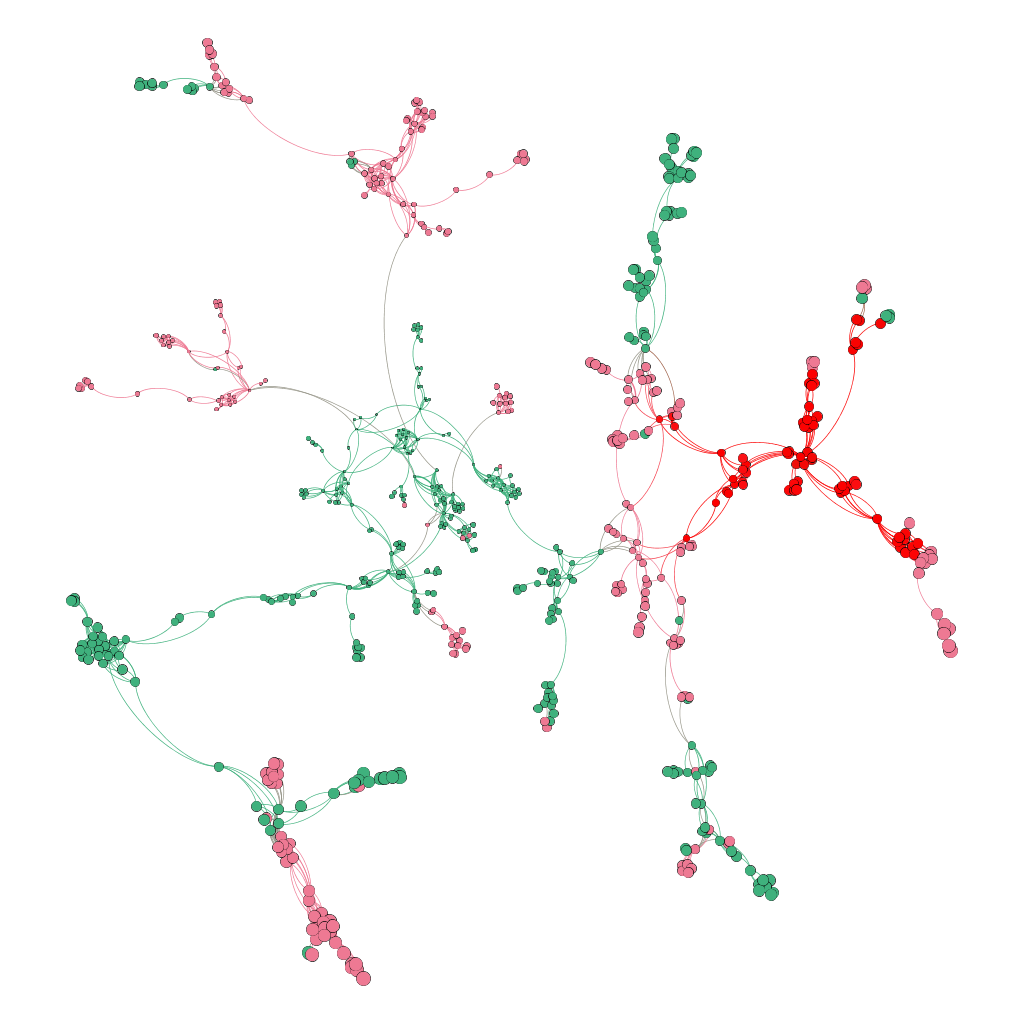
\includegraphics[width=0.52\textwidth]{4.5.png}
        \caption{Node size depending on the eccentricity}
        \label{fig:figure-4.5}
    \end{figure}

\section{Bipartite Graph}
    By considering the original network and removing both the nodes with null degree (done by applying the \textit{degree range} filter with parameter 1 to the maximum) and the edges between companies of the same province (done by applying the \textit{intra-edge} filter as a sub-filter), we obtain the following bipartite graph:

    \begin{figure}[H]
        \centering
        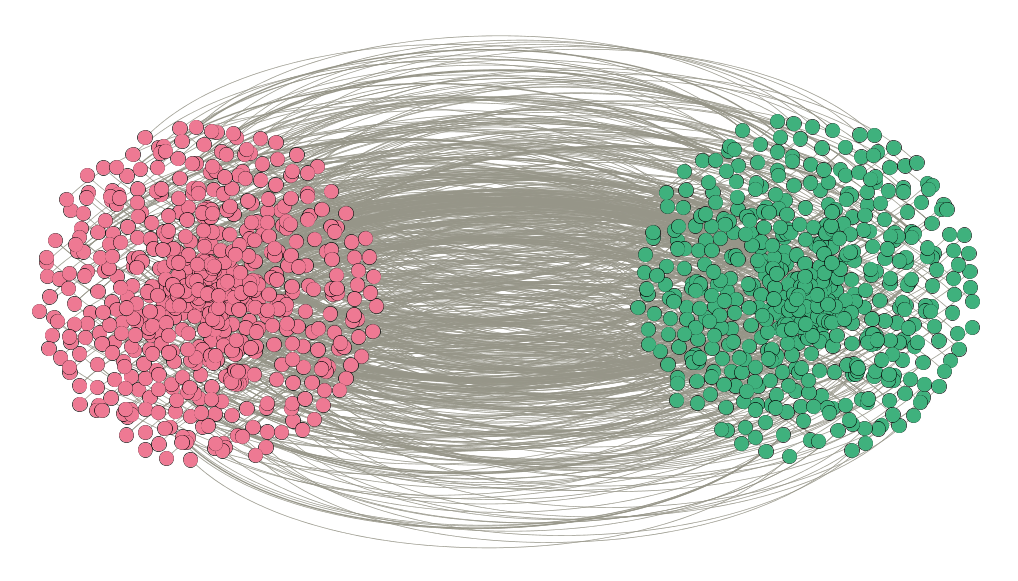
\includegraphics[width=0.65\textwidth]{5.1.png}
        \caption{Bipartite graph}
        \label{fig:figure-5.1}
    \end{figure}

\section{Betweenness Centrality}
    By considering the original network and removing both the nodes with null degree (done by applying the \textit{degree range} filter with parameter 1 to the maximum) and the edges with edge-partition value equal to 1 (done by applying properly the \textit{edge-partition} filter as a sub-filter), we obtain a sub-graph with 1993 nodes and 1471 edges.\newline
    A graphical representation of the obtained bipartite sub-graph can be seen in the 'Figure \ref{fig:figure-6.0}'.
    
    \begin{figure}[H]
        \centering
        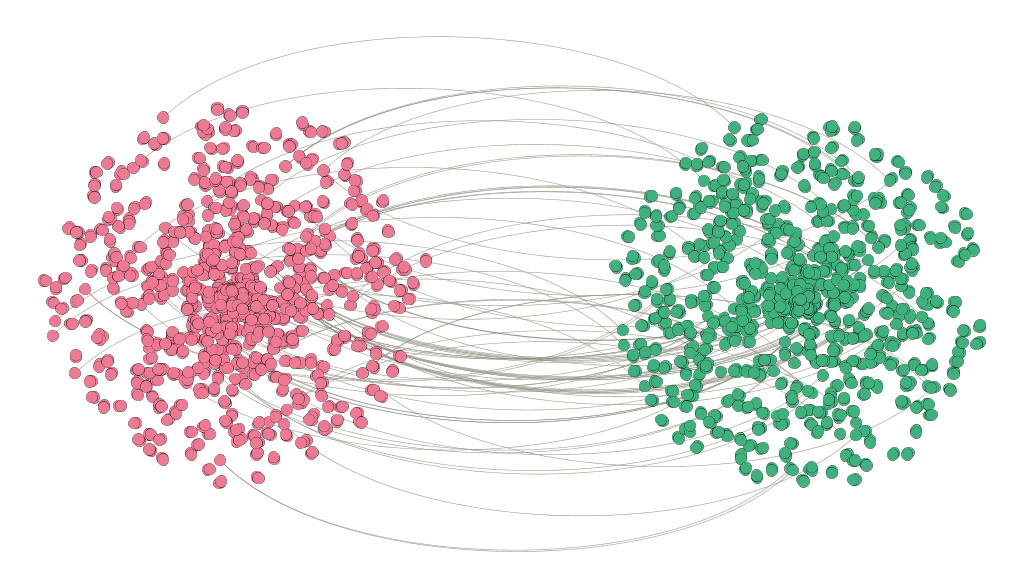
\includegraphics[width=0.65\textwidth]{6.0.png}
        \caption{Bipartite graph}
        \label{fig:figure-6.0}
    \end{figure}
    
    \noindent Moreover the node with the largest betweenness centrality is the one that has its ID equals to 55610 (betweenness centrality = 17.5) and its relative max-depth ego network is:
    
    \begin{figure}[H]
        \centering
        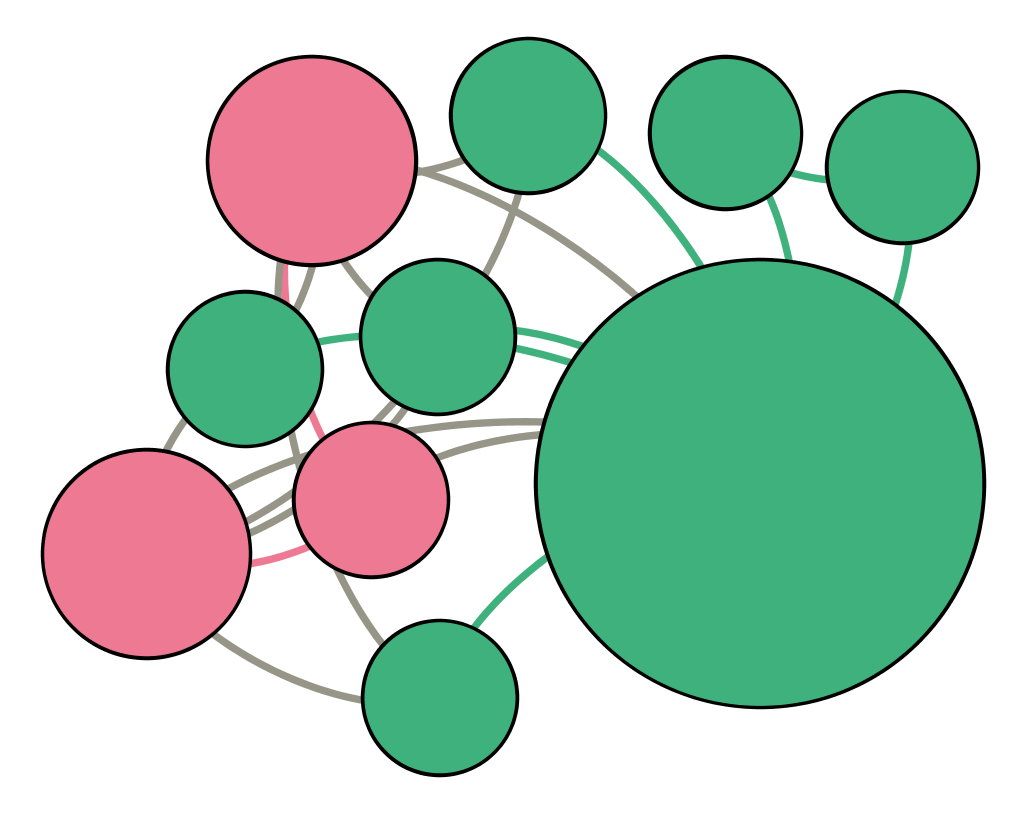
\includegraphics[width=0.4\textwidth]{6.1.png}
        \caption{Max-depth ego network with nodes sizes proportional to their betweenness centrality}
        \label{fig:figure-6.1}
    \end{figure}
    
\section{Additional Notes}
All the data reported in this documentation has been developed using Gephy v0.9.2.\newline
A problem discovered during the tests is that the software didn't recognise properly the imported spreadsheets in such a way that it gave a total of 33340 nodes and 15694 edges (instead of 16896 edges).

\end{document} 